\section{Módulo de Reconhecimento}
\label{sec:modulo_reconhecimento}

	
	Neste módulo é realizada o reconhecimento dos marcadores bem como a obtenção de sua posição na
	imagem do ambiente. Este é notificado a cada imagem nova capturada pela câmera do dispositivo e de
	posse desta sua linha de execução inicia os passos apresentados na figura \ref{fig:processo_detect} e
	conforme descrito a seguir:
	
	\begin{figure}[h]
		\centering 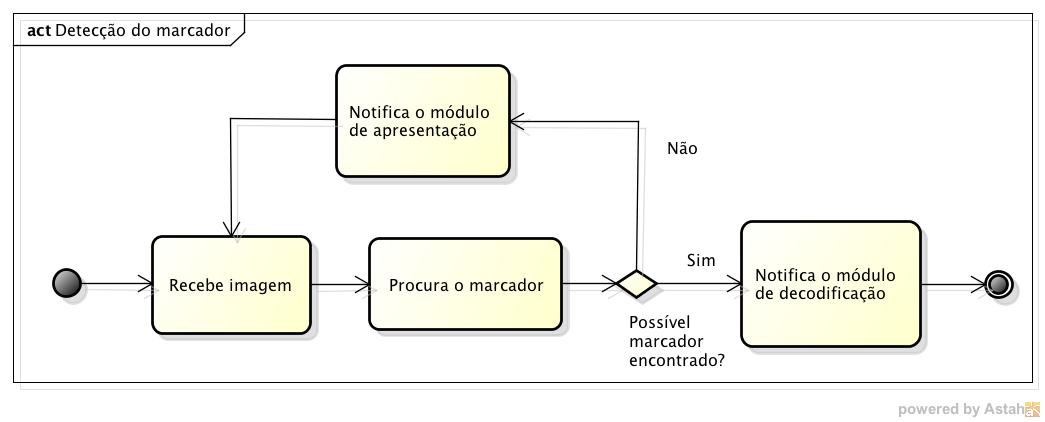
\includegraphics[scale=0.55]{figuras/cap4/processo_deteccao.png}
		\caption{\textit{Processos do Módulo de Reconhecimento.}}
		\label{fig:processo_detect} 
	\end{figure}
	
	\begin{enumerate}

	  \item A imagem obtida é convertida para escala de cinza com o intuito de se obter uma 
	  	homogeneidade da coloração dos \textit{pixels}. Desta forma a detecção de padrões ocorre de forma 
	  	facilitada.
	  
	  \item Utilizando a biblioteca OpenCV é realizada a correção de perspectiva da imagem, já que 
	  	o ângulo observado é distinto da figura esperada (vista frontal). Através da mesma biblioteca 
	  	é realizada a detecção de contornos, com base na borda negra do marcador, e determinação dos 
	  	quatro pontos que a delimitam.
	  	
	  \item Estima-se o posicionamento do marcador baseado nos quatro pontos não lineares
	  		identificados no passo anterior. Nesse procedimento também é obtido o ponto central da imagem,
	  		responsável pelo posicionamento correto do objeto virtual a ser sobreposto ao marcador.
	  
	  \item Para a obtenção da orientação do marcador foi utilizado o sensor de orientação disponível pelo
	  		\textit{smartphone}. A partir dessas informações é possível estimar o ângulo correto de visão
	  		do \textit{smartphone}, posicionando o objeto virtual corretamente.
	  		
	\end{enumerate} 
	
	Caso os quatro passos sejam executados com sucesso, tanto o marcador quanto sua posição seja obtida 
	com sucesso, estas informações são repassadas ao Módulo de Decodificação para que se prossiga com o fluxo 
	normal da aplicação. Caso contrário, é feita uma contagem para analisar se o marcador ainda está sendo 
	capturado pela câmera do celular. Se o processo em andamento atingiu a quantidade máxima de tentativas 
	consecutivas sem sucesso, o Módulo de Apresentação é notificado a respeito que nenhum marcador foi encontrado na 
	imagem, desta forma é possível atualizar a visão do usuário. Independente de ter ocorrido um reconhecimento, 
	o módulo voltará a aguardar	uma nova imagem para que um novo procedimento seja feito.
	
	Apesar da plataforma Android aceitar aplicações que sejam desenvolvidas utilizando a linguagem Java é
	possível combinar aplicações Java com aplicações e bibliotecas desenvolvidas em C/C++. Essa
	integração ocorre através do JNI (\textit{Java Native Interface}) suportada pelo 
	NDK \textit{(Native Development Kit)}. Tirando proveito deste suporte, este módulo integra-se com
	a solução elaborada para o reconhecimento através de uma conexão utilizando o JNI, devido ao fato
	do processo de reconhecimento utilizar a biblioteca \textit{OpenCV}, implementada utilizando a
	linguagem C.
